In this section we will now test the accuracy and the performance of our Inverse Power Method with Deflation algorithm against the \texttt{eigs} function that is natively implemented in MATLAB. As perviously stated our objective is to compute the \(K\) smallest eigenvalues of a symmetric positive semidefinite matrix \(L\).
\\
\\
As benchmark matrix we now use the Laplacian matrix relative to the \texttt{circle} K-NN graph with \(K=10\). For the first benchmark run we computed the 15 smallest eigenvalues and eigenvector using the \texttt{eigs} function in MATLAB and the Inverse power method implemented by us using both the naive deflation method and the Wielandt's deflation method.
\begin{figure}[H]
    \centering
    \subfloat[1][Eigenvalues comparison]{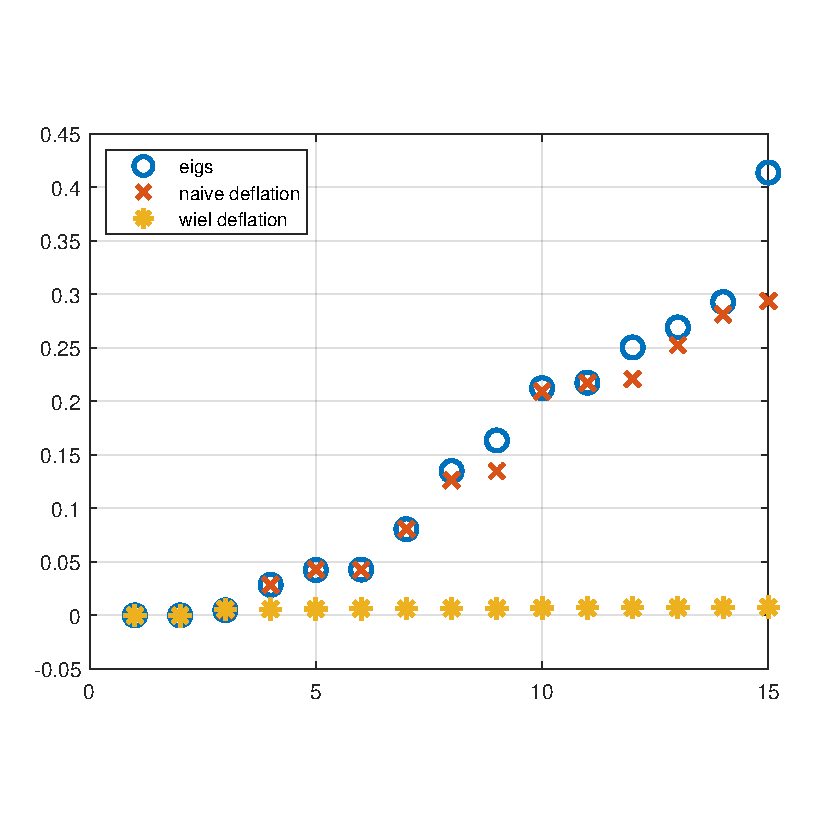
\includegraphics[scale = 0.5]{pictures/ipmd_test/eigenvalues_comp.pdf}}
    \subfloat[2][Partial times to compute eigenvalues in seconds]{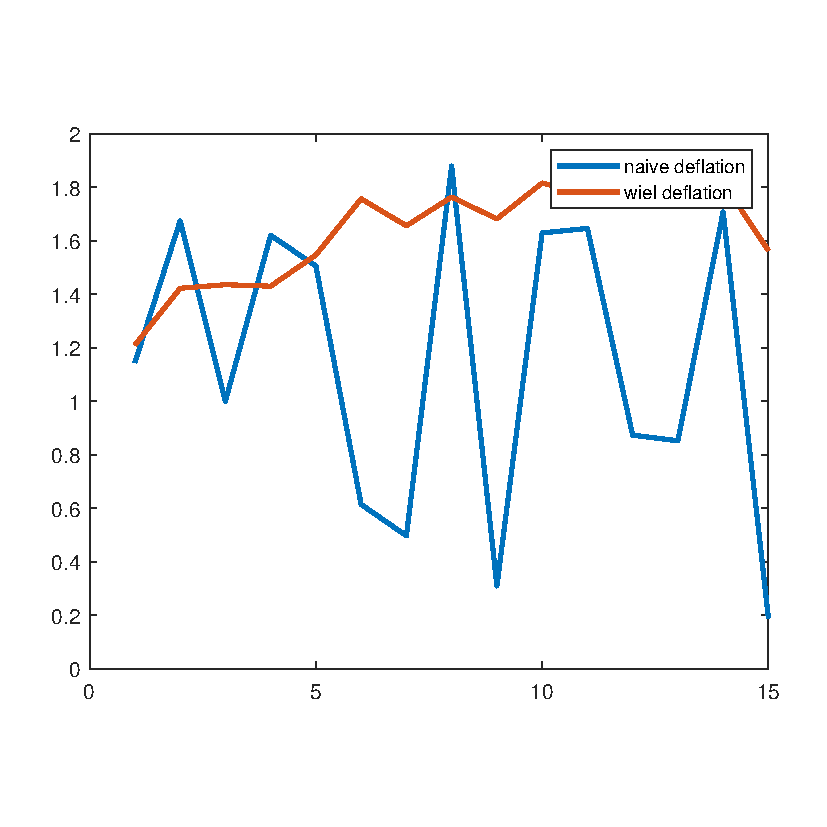
\includegraphics[scale = 0.5]{pictures/ipmd_test/times.pdf}}
    \caption{On the left the comparison between the values of the eigenvalues computed using all methods shown. On the right a plot of the partial times to compute each eigenvalue by using the inverse power method with deflation.}
    \label{Eigenvalues_comp}
\end{figure}
\noindent As we can see clearly in figure \ref{Eigenvalues_comp}, Wielandt deflation performs very badly with respect to the \texttt{eigs} function natively implemented in Matlab for eigenvalue computation. On the other hand, using the naive deflation yielded good results, especially for the first 7 eigenvalues. After some iterations we see that our method for computing eigenvalues is not accurate with respect to the \texttt{eigs} function and this can be attributed to the poor stability of the deflation procedure: at each iteration we are subtracting a rank 1 matrix computed based on an iterative method, and we are propagating potential errors throughout all iterations. 
\begin{figure}[H]
    \centering
    \subfloat[1][\(u_1\)]{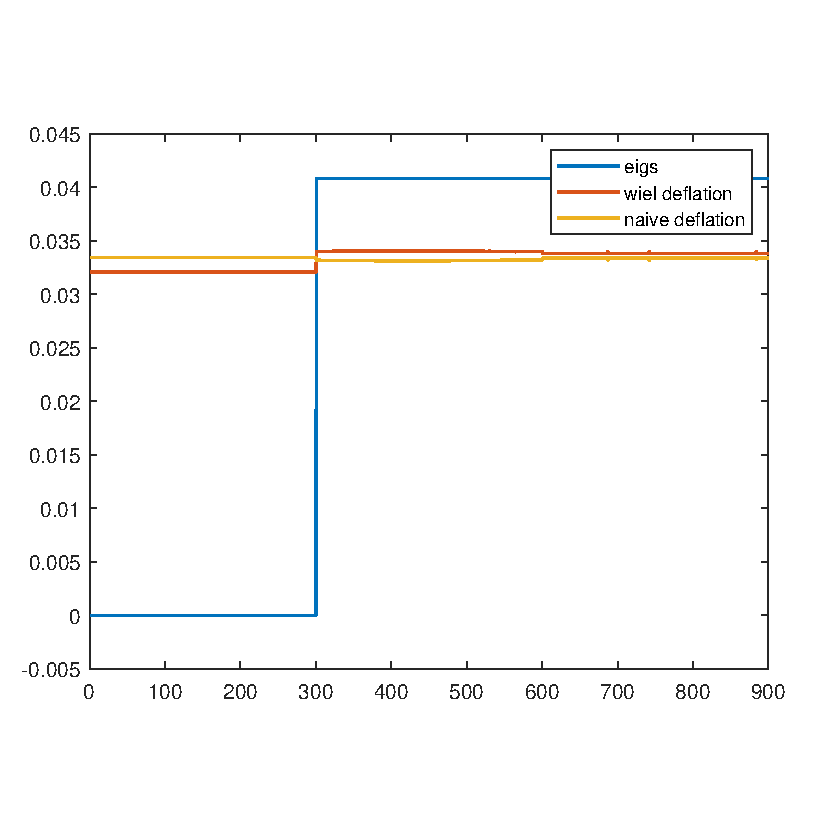
\includegraphics[scale = 0.35]{pictures/ipmd_test/eigenvector_1.pdf}}
    \subfloat[2][\(u_2\)]{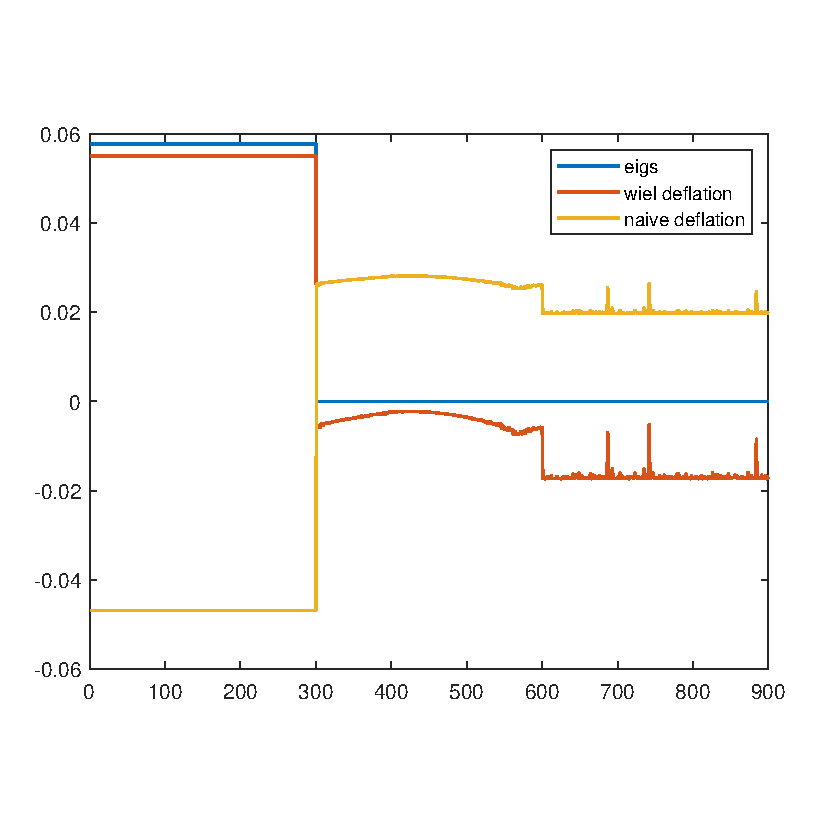
\includegraphics[scale = 0.35]{pictures/ipmd_test/eigenvector_2.pdf}}
    \subfloat[2][\(u_3\)]{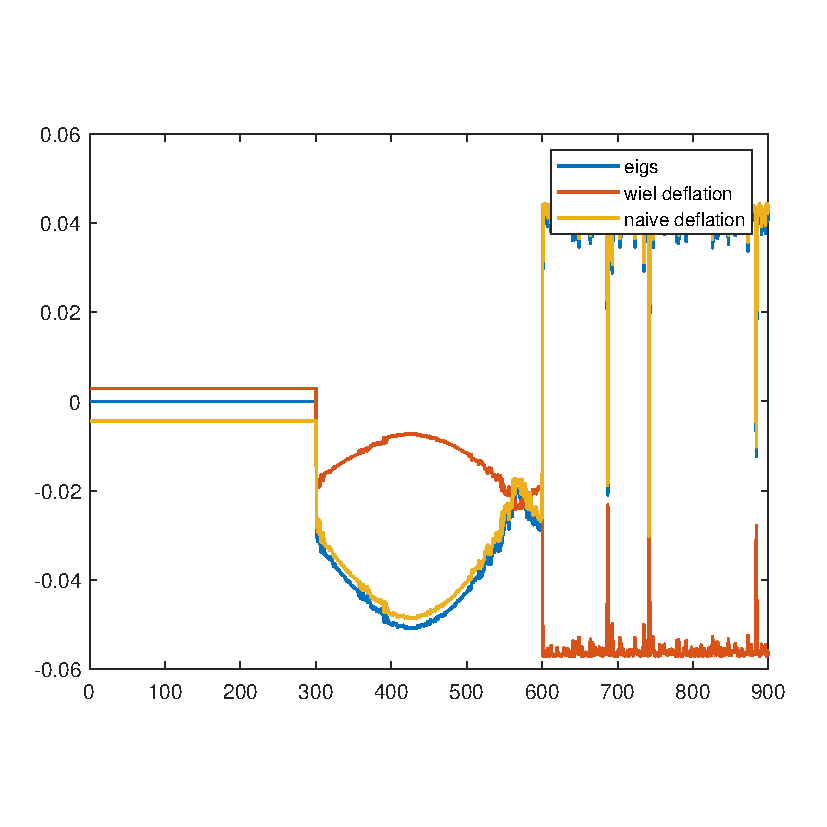
\includegraphics[scale = 0.35]{pictures/ipmd_test/eigenvector_3.pdf}}
    \caption{A plot of the first three eigenvectors computed using the three methods}
    \label{Eigenvectors_comp}
\end{figure}
In figure \ref{Eigenvectors_comp} we plotted the first three eigenvectors computed using the three methods. We can see how each method is able to compute eigenvectors that separate well the clusters of points. As it is clearly visible in the figure, the three clusters of points are well distinguishable using eigenvectors computed with all methods used. This is enforced by the fact that, performing the spectral clustering algorithm using our eigenvalues computation methods, yielded the same results as using the \texttt{eigs} function meaning that we are perfectly able to cluster the points in our benchmark data with our algorithm.


\subsection*{Using the normalized Laplacian matrix}
Using the normalized Laplacian matrix \(L_{\text{sym}} = I - D^{-\frac{1}{2}}WD^{-\frac{1}{2}}\) means that we are shrinking the spectrum of our matrix. We hence expect different results in terms of accuracy of the eigenvalues due to a smaller numerical error since we are comparing at each step numbers in the same order of magnitude.

\begin{figure}[H]
    \centering
    \subfloat[1][Eigenvalues comparison]{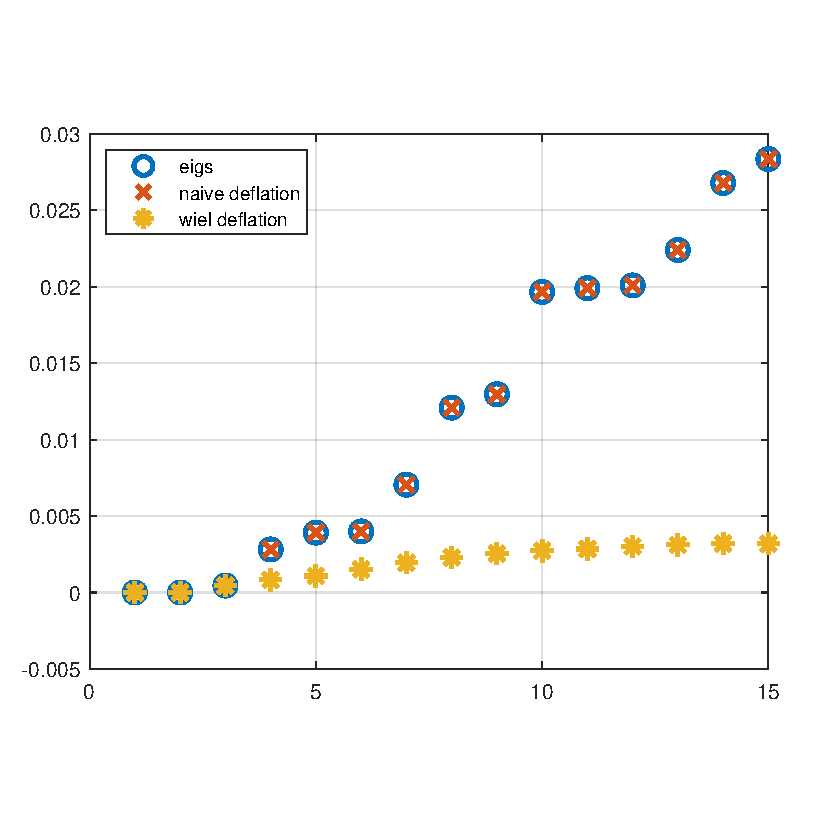
\includegraphics[scale = 0.5]{pictures/ipmd_test/eigenvalues_comp_norm.pdf}}
    \subfloat[2][Partial times to compute eigenvalues in seconds]{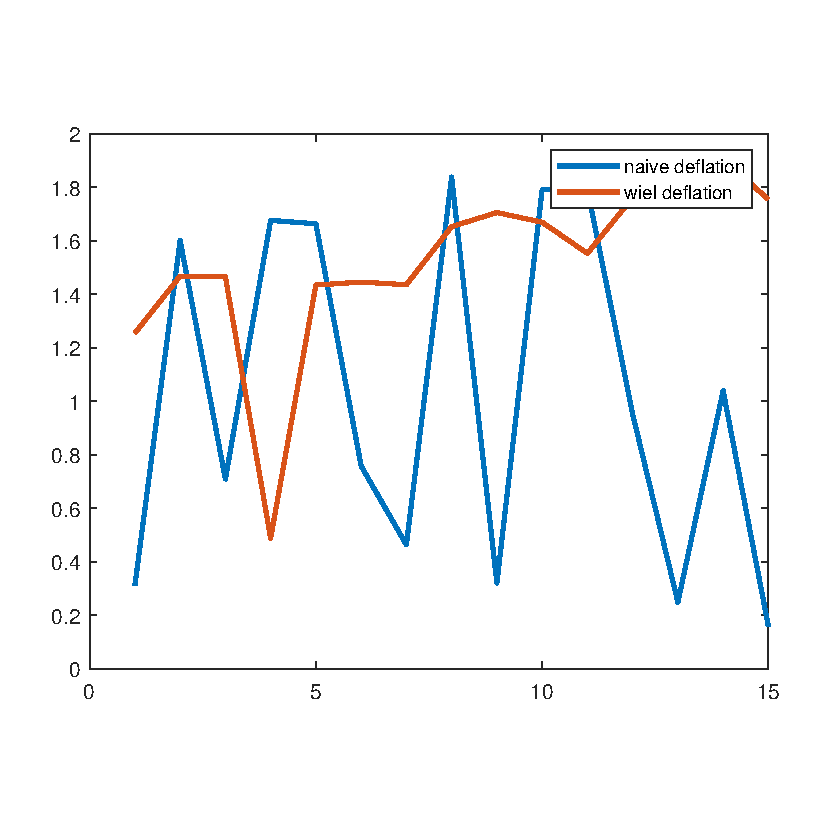
\includegraphics[scale = 0.5]{pictures/ipmd_test/times_norm.pdf}}
    \caption{On the left the comparison between the values of the eigenvalues computed using all methods shown. On the right a plot of the partial times to compute each eigenvalue by using the inverse power method with deflation.}
    \label{Eigenvalues_comp_norm}
\end{figure}

\begin{figure}[H]
    \centering
    \subfloat[1][\(u_1\)]{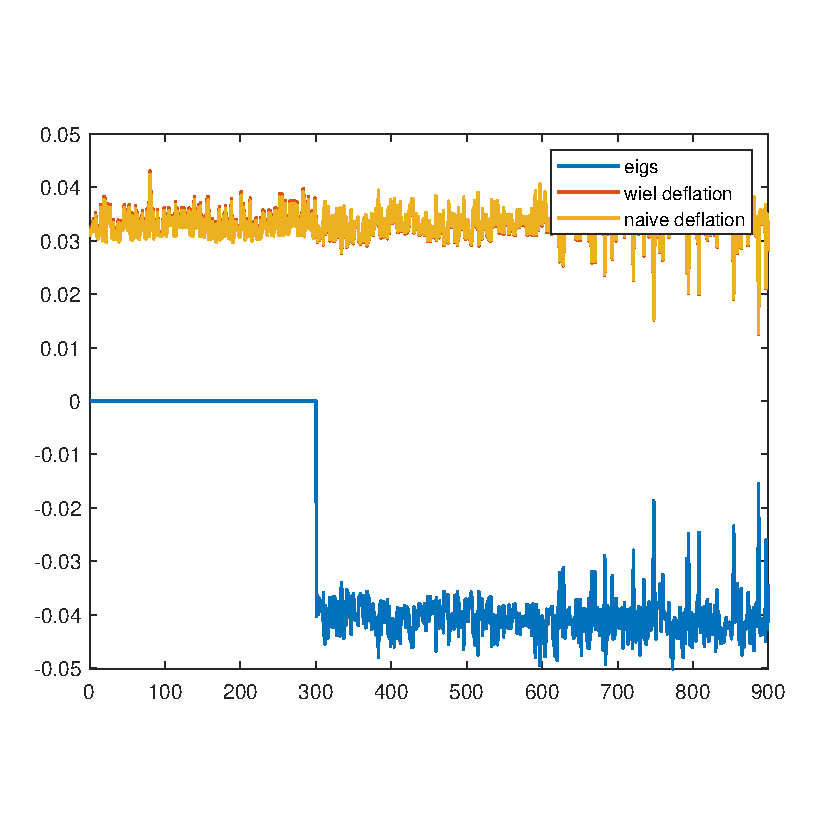
\includegraphics[scale = 0.35]{pictures/ipmd_test/eigenvector_norm_1.pdf}}
    \subfloat[2][\(u_2\)]{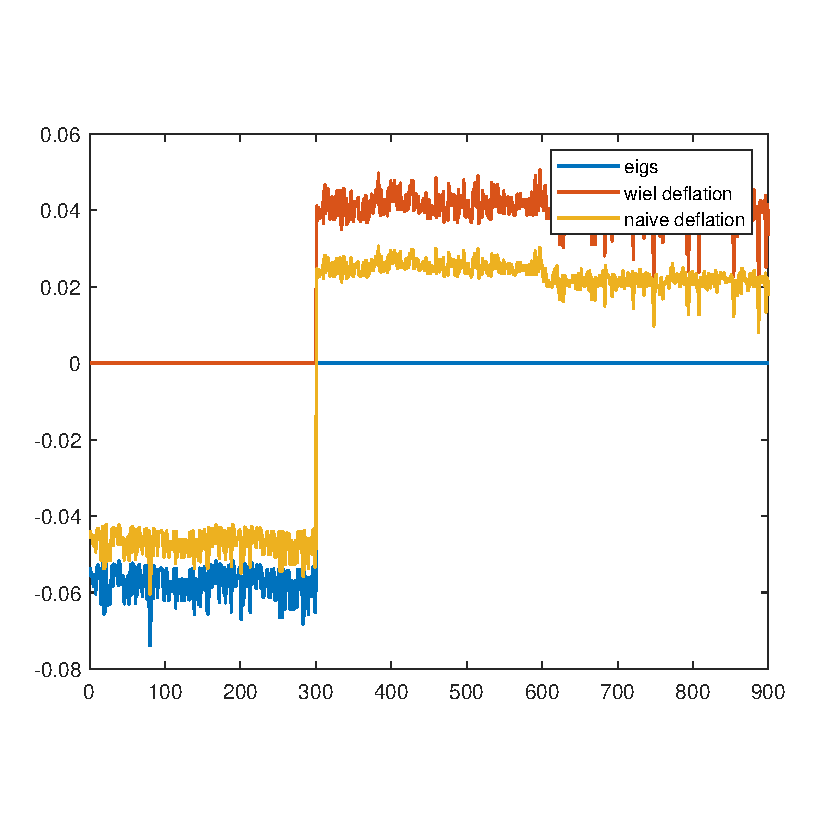
\includegraphics[scale = 0.35]{pictures/ipmd_test/eigenvector_norm_2.pdf}}
    \subfloat[2][\(u_3\)]{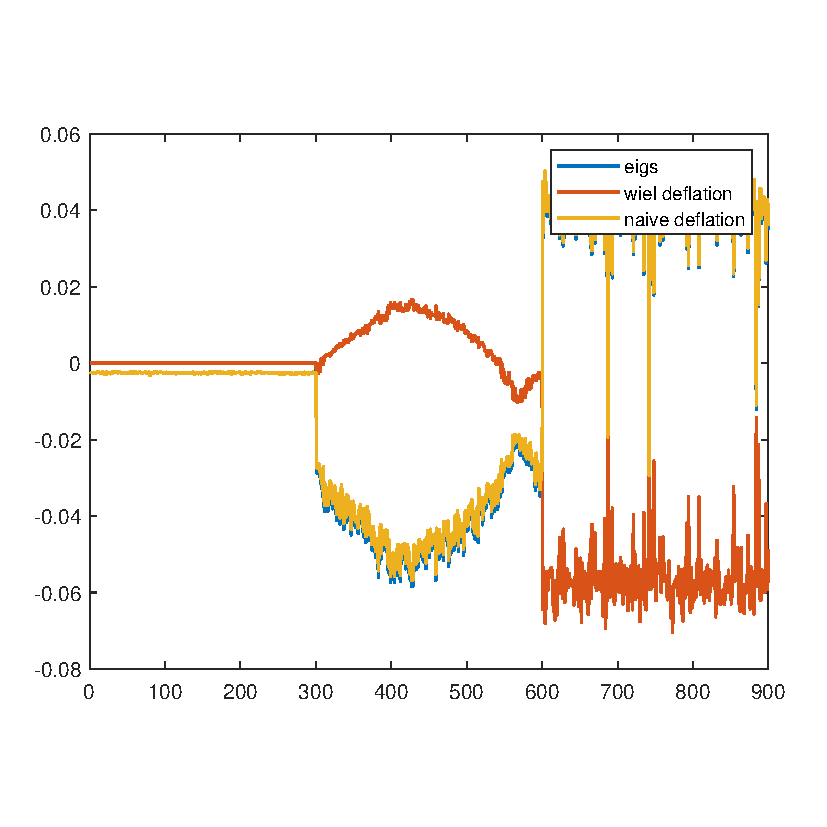
\includegraphics[scale = 0.35]{pictures/ipmd_test/eigenvector_norm_3.pdf}}
    \caption{A plot of the first three eigenvectors computed using the three methods}
    \label{Eigenvectors_comp_norm}
\end{figure}

\noindent In this case the naive deflation technique is much more stable than the unnormalized case. In fact, as we can see in \ref{Eigenvalues_comp_norm}, eigenvalues computed using the naive deflation technique in the inverse power method algorithm are the same as the one computed with the \texttt{eigs} function. As before, Wielandt delfation performs poorly in terms of accuracy with respect to \texttt{eigs}. Nevertheless, all three methods used are able to compute eigenvectors that separate well the cluster of points in our benchmark data, as it is visible in figure \ref{Eigenvectors_comp_norm}. 